\documentclass[aspectratio=169]{beamer}

\usepackage{graphicx}
\usepackage{subfig}
\usepackage{amsmath}
\usepackage{xcolor}

\usetheme{CambridgeUS}
\usecolortheme{dolphin}
% \usecolortheme{beaver}
\AtBeginSection[ ]
{
    \begin{frame}{Outline}
        \tableofcontents[currentsection]
    \end{frame}
}
\title{Denoising Diffusion Probabilistic Models}
\author{
    JinYu\and
    XinkeWang\and
    ChangfengDuan\and
    JieLi\and
    Yuhong Sun}

\institute{ECNU}

\date{\today}

\begin{document}

\begin{frame}
    \titlepage
    \center paper author:
    \centering Jonathan Ho, Ajay Jain, Pieter Abbeel
    \centering -- UC Berkeley
\end{frame}

\begin{frame}{Content}
    \tableofcontents[hideallsubsections]
\end{frame}

\begin{frame}
    \frametitle{Our Team}
    \begin{figure}[htbp]
        \subfloat{
            \begin{minipage}[t]{0.12\linewidth}
                \centering
                
\includegraphics[width=1in]{../pic/dog-pictures/fig0.jpeg}
            \end{minipage}
        }
        \quad
        \subfloat{
            \begin{minipage}[t]{0.12\linewidth}
                \centering
                
\includegraphics[width=1in]{../pic/dog-pictures/fig4.jpeg}
            \end{minipage}
        }
        \quad
        \subfloat{
            \begin{minipage}[t]{0.12\linewidth}
                \centering
                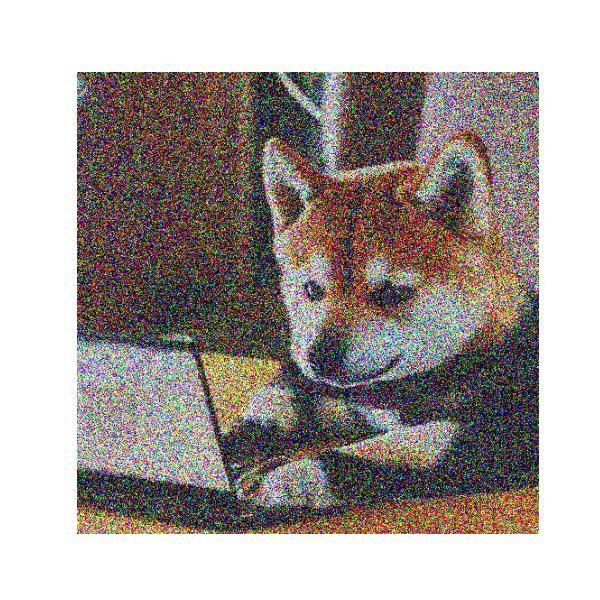
\includegraphics[width=1in]{../pic/dog-pictures/fig10.jpeg}
            \end{minipage}
        }
        \quad
        \subfloat{
            \begin{minipage}[t]{0.12\linewidth}
                \centering
                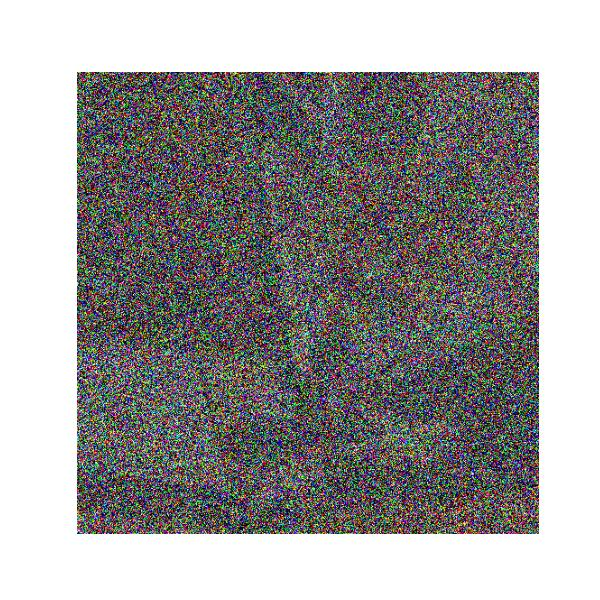
\includegraphics[width=1in]{../pic/dog-pictures/fig14.jpeg}
            \end{minipage}
        }
        \quad
        \subfloat{
            \begin{minipage}[t]{0.12\linewidth}
                \centering
                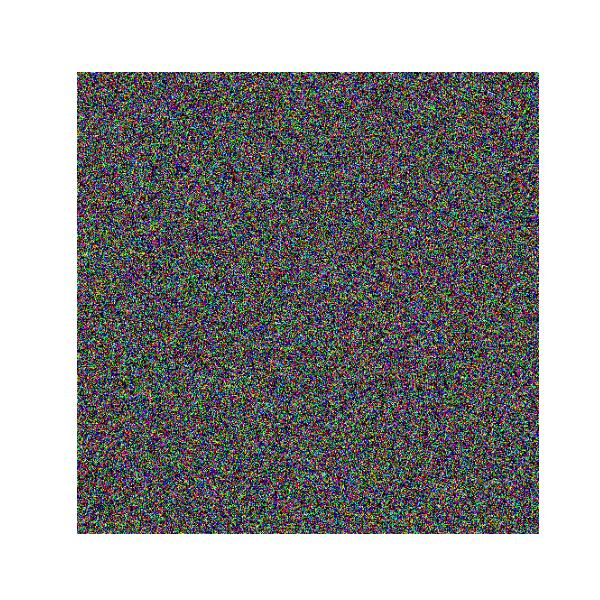
\includegraphics[width=1in]{../pic/dog-pictures/fig19.jpeg}
            \end{minipage}
        }
    \end{figure}

    \ \ \ \ \ \ \ \ \ \ \ \ \ \ \ \ \ \ \ \ \ \
    Yujin\ \ \ \ \ \ \
    XinkeWang\ \ \
    ChangfengDuan\ \ \ \ \ \
    JieLi\ \ \ \ \ \ \ \ \ \
    YuhongSun \ \ \ \ \

\end{frame}


\section{Background}

\begin{frame}{What is generative model?}
    Regardless of precise definition, the terminology is constitutional because a generative model can be used to "generate" random instances
\end{frame}
\begin{frame}{Deep generative models}
    With the rise of deep learning, a new family of methods, called deep generative models (DGMs)
    \begin{itemize}
        \item Generative adversarial networks (GANs)
        \item Variational autoencoders (VAEs)
        \item Flow Based Model
    \end{itemize}
\end{frame}

\section{Introduction}
\begin{frame}{What is Diffusion Model?}
    \begin{block}{We can say...}
        In machine learning, diffusion models, also known as diffusion probabilistic models, are a class of latent variable models.
    \end{block}
\end{frame}

\begin{frame}{Intuitive understanding}
    % picture at here
\end{frame}

\section{Principle}
\begin{frame}{The Process of DDPM}
    \begin{figure}[htbp]
        \centering
        \subfloat[initial]
        {
            \begin{minipage}[b]{.3\linewidth}
                \centering
                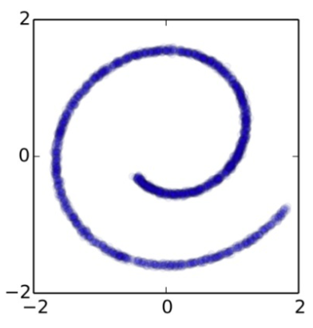
\includegraphics[scale=0.5]{../pic/1.png}
            \end{minipage}
        }
        \subfloat[add noise]
        {
            \begin{minipage}[b]{.3\linewidth}
                \centering
                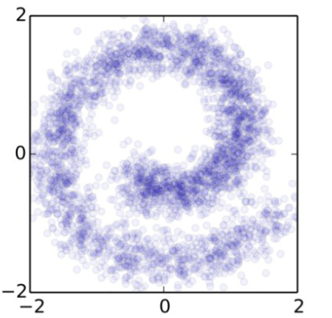
\includegraphics[scale=0.5]{../pic/2.png}
            \end{minipage}
        }
        \subfloat[final]
        {
            \begin{minipage}[b]{.3\linewidth}
                \centering
                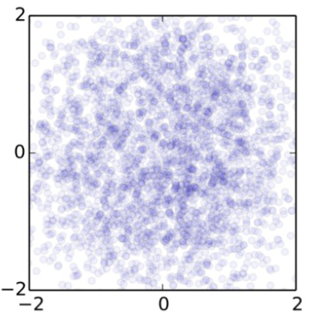
\includegraphics[scale=0.5]{../pic/3.png}
            \end{minipage}
        }
        \caption{how the figure tranform to a Gaussian Distribution}
    \end{figure}
\end{frame}

\begin{frame}{Formula}
    \begin{block}{Forward}
        \begin{equation}
            q(x_t|x_{t-1}) = N(x_t;x_{t-1}\sqrt{1-\beta t}, I\beta_t)
        \end{equation}
        \begin{equation}
            x_t = x_{t-1} \sqrt{1-\beta_t} +  z_t\sqrt{\beta_t}
        \end{equation}
    \end{block}
    \begin{block}{Backward}
        \begin{equation}
            p(x_t|x_{t-1}) = N(x_{t-1};f_\mu(x_t, t),f_\sigma(x_t, t))
        \end{equation}
    \end{block}
\end{frame}

\begin{frame}{Forward Equation}
    \begin{align*}
        x_t & = x_{t-1} \sqrt{1-\beta_t}+ z_t\sqrt{\beta_t} \ \ \ ({\rm let\ } 1-\beta_t = \alpha_t) \tag{1a}                              \\
            & = x_{t-2} \sqrt{\alpha_t}(\sqrt{\alpha_{t-1}} + z_{t-2} \sqrt{1-\alpha_{t-1}}) + z_{t-1}\sqrt{1-\alpha_t}   \tag{2a}         \\
            & = x_{t-2} \sqrt{\alpha_t\alpha_{t-1}}  + z_{t-2} \sqrt{\alpha_t - \alpha_t\alpha_{t-1}} + z_{t-1} \sqrt{1-\alpha_t} \tag{3a} \\
            & = x_{t-2} \sqrt{\alpha_t\alpha_{t-1}} + z\sqrt{1-\alpha_t\alpha_{t-1}}                                          \tag{4a}     \\
            & = \cdots                                                                                                                     \\
            & = x_0 \sqrt{\bar{\alpha_t}} + z\sqrt{1-\bar{\alpha_t}}\tag{5a}
    \end{align*}
\end{frame}


\begin{frame}
    \frametitle{Backward Equation}
    \begin{align*}
        q(x_{t-1} | x_t, x_0) & = q(x_t | x_{t-1}, x_0) \frac{q(x_{t-1}|x_0)}{q(x_t|x_0)} \\
                              & \propto \exp\left(
        - \frac 12 \left(
        \textcolor{red} { (\frac{\alpha_t}{\beta_t}
            + \frac 1{1-\bar{\alpha}_{t-1}}) } x_{t-1}^2
        \textcolor{blue}{ - (\frac{2\sqrt{\alpha_t}}{\beta_t}x_t
            + \frac{2\sqrt{\bar{\alpha}_{t-1}}} {1-\bar{\alpha}_{t-1}} )} x_{t-1}
        +C(x_t, x_0) \right)
        \right)                                                                           \\
                              & = \exp \left ( -\frac12
        \left ( \textcolor{red}{A} x_{t-1}^2 + \textcolor{blue}{B} x_{t-1} + C \right )
        \right )
    \end{align*}
    \begin{equation}
        E (x_{t-1}) = -\frac{\textcolor{blue}{B}}{2\textcolor{red}{A}}, Var(x_{t-1}) = \frac {1}{\textcolor{red}{A}}
    \end{equation}
\end{frame}
\section{Advantage}

\begin{frame}{DDPM Advantage}
    \begin{table}
        \begin{tabular}{| c || c | c | c | c | c |  }
            \hline
            Name.      & Quality & Likelihood & Speed & Gradually or One-time & Stability \\
            \hline \hline
            GAN        & ++      & Uncertain  & fast  & One-time              & Unstable  \\
            VAE        & ++      & Uncertain  & fast  & One-time              & -         \\
            Flow Model & +       & Certain    & fast  & Gradually             & -         \\
            DDPM       & +++     & -          & slow  & Gradually             & Stable    \\
            \hline
        \end{tabular}
        \caption{cons and pros of generative model}
    \end{table}
\end{frame}

\section{Application}

\begin{frame}{Text2Image}
    \centering
    
\includegraphics[height=4.5cm]{../pic/dog-is-reading.png}
\end{frame}
\begin{frame}{Image refinement}
    \centering
    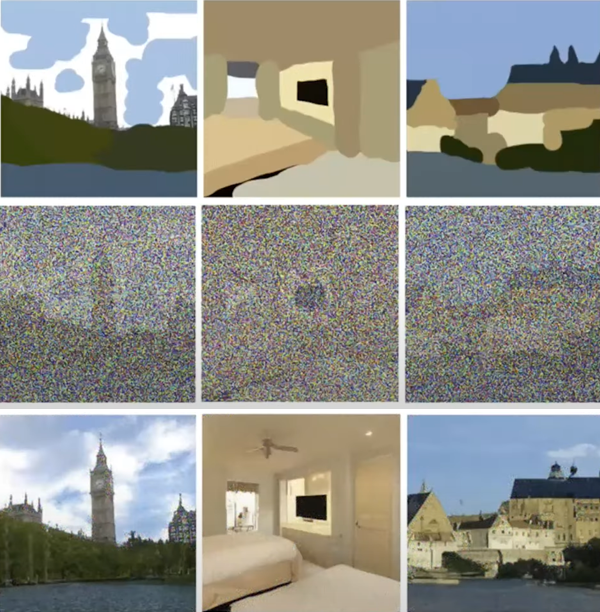
\includegraphics[height=4.5cm]{../pic/compose.png}
\end{frame}
\begin{frame}{Inpainting}
    \centering
    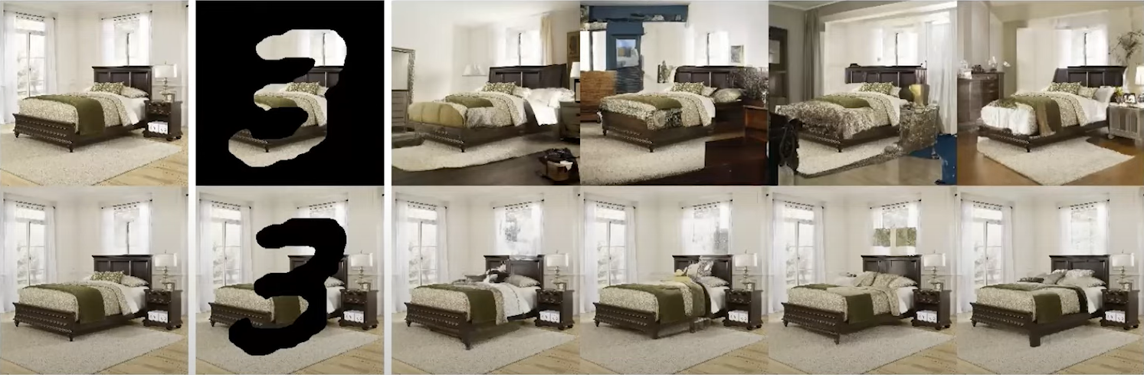
\includegraphics[height=4.5cm]{../pic/inpainting.png}
\end{frame}
\begin{frame}{Colorization}
    \centering
    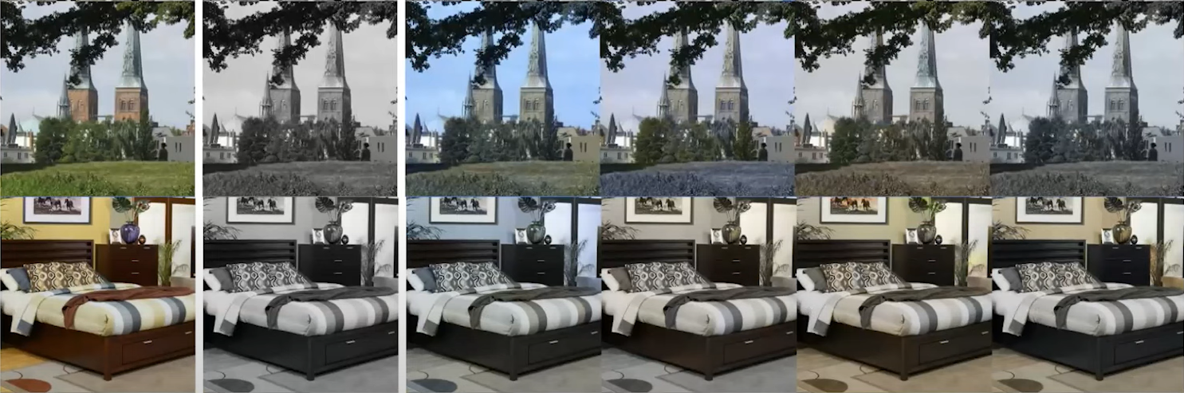
\includegraphics[height=4.5cm]{../pic/colorization.png}
\end{frame}
\begin{frame}{Conclusion}

\end{frame}

\section{Reference}
\begin{frame}{Reference}
    Thanks\\
    \LaTeX
\end{frame}

\end{document}